\documentclass[10pt,aspectratio=169]{beamer}

% ---------- packages ----------
\usepackage[T1]{fontenc}
\usepackage[utf8]{inputenc}
\usepackage{lmodern}
\usepackage{amsmath,amssymb}
\usepackage{tikz}
\usepackage{pgfplots}
\pgfplotsset{compat=1.17}
\usetikzlibrary{arrows.meta,positioning,fit,backgrounds,decorations.pathreplacing,calc}
\usepackage{booktabs}
\usepackage{array}
\usepackage{xcolor}

% ---------- bare theme, built by hand ----------
\usetheme{default}
\setbeamertemplate{navigation symbols}{}
\beamertemplatenavigationsymbolsempty

\renewcommand{\familydefault}{\sfdefault}

% palette
\definecolor{inkNavy}{HTML}{102A43}
\definecolor{slate}{HTML}{334E68}
\definecolor{paleBg}{HTML}{F0F4F8}
\definecolor{amberAccent}{HTML}{C98A1B}
\definecolor{tealAccent}{HTML}{1B7A72}
\definecolor{cardBlue}{HTML}{E3ECF5}
\definecolor{cardAmber}{HTML}{FBF0DD}
\definecolor{cardGray}{HTML}{ECEFF3}
\definecolor{cardTeal}{HTML}{E1F0EE}
\definecolor{softRed}{HTML}{9E2A2B}

\setbeamercolor{normal text}{fg=inkNavy,bg=white}
\setbeamercolor{structure}{fg=inkNavy}
\setbeamercolor{frametitle}{fg=inkNavy,bg=white}
\setbeamercolor{title}{fg=inkNavy}
\setbeamercolor{author}{fg=slate}
\setbeamercolor{date}{fg=slate}
\setbeamercolor{footline}{fg=slate}
\setbeamercolor{itemize item}{fg=amberAccent}
\setbeamercolor{itemize subitem}{fg=tealAccent}
\setbeamercolor{block title}{fg=inkNavy,bg=cardBlue}
\setbeamercolor{block body}{fg=inkNavy,bg=cardBlue!40}
\setbeamercolor{cardblue box}{fg=inkNavy,bg=cardBlue}
\setbeamercolor{cardamber box}{fg=inkNavy,bg=cardAmber}
\setbeamercolor{cardgray box}{fg=inkNavy,bg=cardGray}
\setbeamercolor{cardteal box}{fg=inkNavy,bg=cardTeal}

\setbeamerfont{frametitle}{series=\bfseries,size=\Large}
\setbeamerfont{title}{series=\bfseries}
\setbeamertemplate{itemize item}{\raisebox{0.15em}{\scalebox{0.55}{\textbullet}}}
\setbeamertemplate{itemize subitem}{\raisebox{0.1em}{\scalebox{0.5}{$\blacktriangleright$}}}

% frame title with a thin rule
\setbeamertemplate{frametitle}{
  \vspace{0.35em}
  {\usebeamerfont{frametitle}\usebeamercolor[fg]{frametitle}\insertframetitle}
  \par\vspace{0.25em}
  {\color{amberAccent}\rule{\linewidth}{1.6pt}}
}

% footline: page count
\setbeamertemplate{footline}{
  \leavevmode
  \hbox{
    \begin{beamercolorbox}[wd=.5\paperwidth,ht=2.6ex,dp=1.2ex,left,leftskip=1em]{footline}
      \tiny\color{slate} fracmem \; \textbar\; technical overview
    \end{beamercolorbox}
    \begin{beamercolorbox}[wd=.5\paperwidth,ht=2.6ex,dp=1.2ex,right,rightskip=1em]{footline}
      \tiny\color{slate} \insertframenumber\,/\,\inserttotalframenumber
    \end{beamercolorbox}
  }
}

% custom card environments
\newcommand{\ideacard}[1]{%
  \begin{beamercolorbox}[wd=\linewidth,sep=0.9em,rounded=true]{cardamber box}
  {\color{amberAccent}\textbf{Key idea.}} #1
  \end{beamercolorbox}}

\newcommand{\saycard}[1]{%
  \begin{beamercolorbox}[wd=\linewidth,sep=0.9em,rounded=true]{cardteal box}
  #1
  \end{beamercolorbox}}

\title{\textbf{fracmem}}
\subtitle{Technical Overview}
\author{Adithyan Lalu}
\institute{Guidance, Navigation \& Control \textbar\ Autonomous Systems}
\date{\today}

\begin{document}

% ---------------------------------------------------------------- title
{
\setbeamertemplate{footline}{}
\begin{frame}[plain]
  \vspace{1.1cm}
  \begin{center}
    {\Huge\bfseries\color{inkNavy} fracmem}\\[0.6em]
    {\large\color{slate} Compressed Fractional Order Memory}\\[0.3em]
    {\footnotesize\color{slate} Constant time, constant memory filters for fractional order systems}\\[1.6em]
    {\color{amberAccent}\rule{0.5\linewidth}{1.4pt}}\\[1.6em]
    {\large Adithyan Lalu}\\[0.25em]
    {\small\color{slate} Guidance, Navigation \& Control \textbar\ Autonomous Systems}\\[0.3em]
    {\small\color{slate} \today}
  \end{center}
\end{frame}
}

% ---------------------------------------------------------------- outline
\begin{frame}{Overview}
  \begin{enumerate}
    \setlength\itemsep{0.85em}
    \item Motivation and the core challenge
    \item Solution approach, in three steps
    \item Formulation behind each step
    \item Validation: accuracy and performance
    \item Deployment targets
  \end{enumerate}
\end{frame}

% ---------------------------------------------------------------- why this exists
\begin{frame}{Motivation}
  An ordinary derivative only cares about what just happened.

  \vspace{0.3em}
  \saycard{A \textbf{fractional order} derivative is different: it needs to remember \emph{everything} that has ever happened, with old events fading away slowly instead of being forgotten. This shows up in fractional order control systems, aircraft and drone dynamics, materials that slowly deform, and batteries.}

  \vspace{0.4em}
  The problem: remembering everything, the naive way, costs a little more compute every single step, forever. On a real microcontroller with fixed memory and a fixed time budget, that eventually breaks.

  \vspace{0.3em}
  \ideacard{fracmem replaces "remember everything" with a small, fixed size trick that never grows, no matter how long it runs.}
\end{frame}

% ---------------------------------------------------------------- the problem visually
\begin{frame}{The Core Challenge}
  \begin{columns}[T]
    \begin{column}{0.5\linewidth}
      \vspace{0.6em}
      An ordinary system forgets fast. A fractional order system forgets \emph{very} slowly, so cutting its memory short throws away real accuracy.

      \vspace{0.6em}
      \saycard{This slow fading is not a flaw to fix, it is the actual behavior fractional order systems have. The trick is representing it cheaply, not skipping it.}
    \end{column}
    \begin{column}{0.5\linewidth}
      \begin{center}
      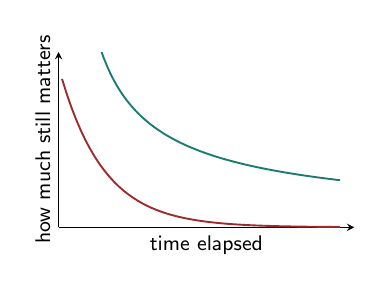
\begin{tikzpicture}[scale=0.85]
        \begin{axis}[
          width=6cm, height=4.2cm,
          xlabel={\small time elapsed}, ylabel={\small how much still matters},
          xmin=0, xmax=4.2, ymin=0, ymax=2.4,
          axis lines=left, tick label style={font=\tiny},
          label style={font=\small}, ticks=none
        ]
        \addplot[domain=0.05:4, samples=60, thick, softRed] {2.2*exp(-1.6*x)};
        \addplot[domain=0.15:4, samples=80, thick, tealAccent] {1.7*(x)^(-0.7)};
        \end{axis}
      \end{tikzpicture}\\[0.2em]
      {\small\color{softRed}\textbf{ordinary}: forgets fast} \quad {\small\color{tealAccent}\textbf{fractional order}: forgets slowly}
      \end{center}
    \end{column}
  \end{columns}
\end{frame}

% ---------------------------------------------------------------- the formula
\begin{frame}{The Governing Equation}
  \small First, the pieces: $x$ is the signal you are measuring (say, a sensor reading), $x_{k-j}$ means "the value of $x$, $j$ steps before now", and $\alpha$ is just a number you pick, like $0.5$, that says how "fractional" the derivative is.

  \vspace{0.3em}
  With those pieces, a fractional order derivative is written as:
  \[
  \underbrace{D^\alpha x(t_k)}_{\substack{\text{the answer}\\\text{we want, right now}}} \;\approx\; \underbrace{h^{-\alpha}}_{\substack{\text{a fixed}\\\text{rescaling number}}} \underbrace{\sum_{j=0}^{k} w_j\, x_{k-j}}_{\text{add up the entire past, weighted}}
  \]
  where $w_j$ is one fixed weight per step $j$, a number that shrinks the further back $j$ points, so recent moments count more than distant ones.

  \vspace{0.3em}
  \ideacard{The catch: "the entire past" means this sum has more and more terms to add every single step, forever. That growing sum is exactly the problem fracmem exists to solve.}
\end{frame}

% ---------------------------------------------------------------- big picture
\begin{frame}{Solution Approach}
  \begin{center}
  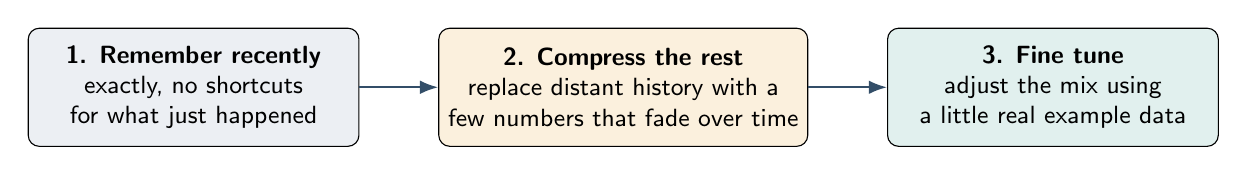
\begin{tikzpicture}[node distance=0.6cm, every node/.style={font=\small, align=center}]
    \node[draw, rounded corners, fill=cardGray, minimum width=4.2cm, minimum height=1.5cm] (a) {\textbf{1. Remember recently}\\exactly, no shortcuts\\for what just happened};
    \node[draw, rounded corners, fill=cardAmber, right=1cm of a, minimum width=4.2cm, minimum height=1.5cm] (b) {\textbf{2. Compress the rest}\\replace distant history with a\\few numbers that fade over time};
    \node[draw, rounded corners, fill=cardTeal, right=1cm of b, minimum width=4.2cm, minimum height=1.5cm] (c) {\textbf{3. Fine tune}\\adjust the mix using\\a little real example data};
    \draw[-{Latex}, thick, slate] (a) -- (b);
    \draw[-{Latex}, thick, slate] (b) -- (c);
  \end{tikzpicture}
  \end{center}

  \vspace{0.6em}
  \ideacard{Steps 1 and 2 come from pure mathematics, worked out once, ahead of time. Step 3 is the only place real data comes in, just to polish an answer that is already close.}

  \vspace{0.4em}
  \centering\small\color{slate} The following slides detail the formulation and validation for each step.
\end{frame}

% ---------------------------------------------------------------- step 1
\begin{frame}{Step 1 \textbar\ Exact Recent Window}
  \begin{center}
  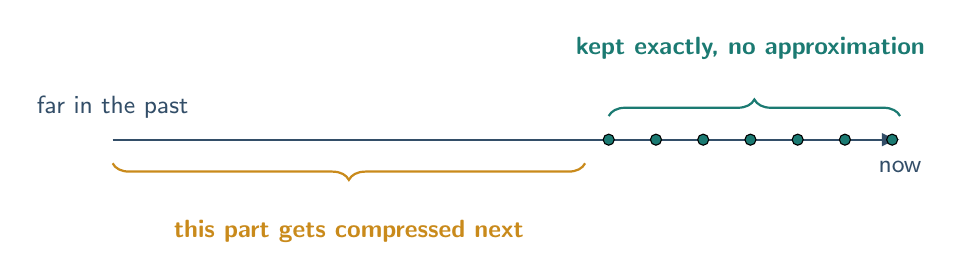
\begin{tikzpicture}[every node/.style={font=\small}]
    \draw[thick, slate, -{Latex}] (0,0) -- (10,0);
    \node[above, slate] at (0,0.15) {far in the past};
    \node[below, slate] at (10,-0.15) {now};
    \draw[decorate, decoration={brace, amplitude=6pt}, thick, tealAccent] (6.3,0.3) -- (10,0.3);
    \node[above, tealAccent, font=\small\bfseries] at (8.1,0.9) {kept exactly, no approximation};
    \draw[decorate, decoration={brace, amplitude=6pt, mirror}, thick, amberAccent] (0,-0.3) -- (6,-0.3);
    \node[below, amberAccent, font=\small\bfseries] at (3,-0.9) {this part gets compressed next};
    \foreach \x in {6.3,6.9,...,10} \draw[fill=tealAccent] (\x,0) circle (2pt);
  \end{tikzpicture}
  \end{center}

  \vspace{1.2em}
  \saycard{The most recent handful of moments are kept and used exactly as they are, an ordinary, simple running window. No approximation happens here at all. Everything older than that is where the real trick is needed.}
\end{frame}

% ---------------------------------------------------------------- step 2
\begin{frame}{Step 2 \textbar\ Compressed Long Term Memory}
  \saycard{Imagine a few small counters. Every new moment tops each counter up a little. Between updates, every counter also fades, a bit like a dimmer light slowly going darker. Add up what is left in all the counters, and that single number stands in for the entire distant past.}

  \vspace{0.15em}
  \begin{center}
  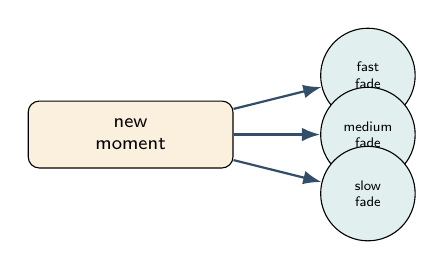
\begin{tikzpicture}[node distance=0.55cm and 0.7cm]
    \node[draw, rounded corners, fill=cardAmber, minimum width=2.6cm, minimum height=0.85cm, font=\scriptsize, align=center] (in) {new\\moment};
    \node[draw, circle, fill=cardTeal, right=1.1cm of in, minimum size=1.2cm, font=\tiny, align=center, yshift=0.75cm] (b1) {fast\\fade};
    \node[draw, circle, fill=cardTeal, right=1.1cm of in, minimum size=1.2cm, font=\tiny, align=center] (b2) {medium\\fade};
    \node[draw, circle, fill=cardTeal, right=1.1cm of in, minimum size=1.2cm, font=\tiny, align=center, yshift=-0.75cm] (b3) {slow\\fade};
    \draw[-{Latex}, thick, slate] (in) -- (b1);
    \draw[-{Latex}, thick, slate] (in) -- (b2);
    \draw[-{Latex}, thick, slate] (in) -- (b3);
  \end{tikzpicture}
  \end{center}

  \vspace{0.2em}
  \ideacard{How fast each counter fades is never guessed or trial and errored: an exact mathematical formula picks the fading speeds, before any real signal is seen.}
\end{frame}

% ---------------------------------------------------------------- step 2 math
\begin{frame}{Step 2 \textbar\ Formulation}
  \small One counter, updated every step by one simple rule:
  \[
  \underbrace{m[k]}_{\substack{\text{counter's value,}\\\text{right now}}} \;=\; \underbrace{\lambda}_{\substack{\text{fading speed,}\\\text{a number 0 to 1}}} \cdot \underbrace{m[k-1]}_{\substack{\text{counter's value,}\\\text{one step ago}}} \;+\; \underbrace{x[k]}_{\substack{\text{newest signal}\\\text{sample}}}
  \]
  In words: keep a fraction $\lambda$ of what the counter already held, then add the newest sample. A small $\lambda$ fades fast, a $\lambda$ near 1 fades slowly.

  \vspace{0.3em}
  Now use a handful of these counters at once, say $p$ of them, each with its own speed. Label them $m_1[k], m_2[k], \dots$, and give each one a mixing amount $c_1, c_2, \dots$, a number saying how much that counter counts. Add them all up:
  \[
  \underbrace{\hat T[k]}_{\text{our stand in for the far past}} \;=\; \underbrace{c_1 m_1[k] + c_2 m_2[k] + \cdots}_{\text{each counter, times how much it counts}}
  \]
  \small\color{slate} The speeds ($\lambda_1,\lambda_2,\dots$) come from an exact formula, decided once. The mixing amounts ($c_1,c_2,\dots$) are exactly what step 3 figures out next.
\end{frame}

% ---------------------------------------------------------------- step 3
\begin{frame}{Step 3 \textbar\ Data Driven Calibration}
  Once the fading speeds are locked in by pure math, one question is left: how much should each counter count?

  \vspace{0.4em}
  \saycard{That is answered with a small amount of real example data, a handful of representative signals, not a huge dataset. Finding the best mix is an easy, always solvable fitting problem, similar to finding the best blend of ingredients from a few taste tests: there is always exactly one best answer, and it can be found directly, with no guessing and no trial and error.}

  \vspace{0.4em}
  \ideacard{Why not also let data choose the fading speeds? Because those already have a provably correct answer from pure math. Only the mixing amounts genuinely benefit from seeing real data.}
\end{frame}

% ---------------------------------------------------------------- step 3 math
\begin{frame}{Step 3 \textbar\ Formulation}
  \small Recall from step 2: the mixing amounts $c_1, c_2, \dots$ are the only unknowns left. Here is how they get found.

  \vspace{0.3em}
  Run the counters on a few example signals where the true answer is already known. For every moment $k$ in those examples, you now have two things: what each counter read, and what the answer should have been:

  \begin{center}
  \small
  \begin{tabular}{ccccc}
    \toprule
    moment & counter 1 & counter 2 & counter 3 & true answer \\
    \midrule
    $k{=}1$ & 0.8 & 0.3 & 0.1 & 0.52 \\
    $k{=}2$ & 0.6 & 0.5 & 0.2 & 0.48 \\
    $\vdots$ & $\vdots$ & $\vdots$ & $\vdots$ & $\vdots$ \\
    \bottomrule
  \end{tabular}
  \end{center}

  \vspace{0.3em}
  \saycard{The question becomes: what $c_1, c_2, c_3$ make $c_1(\text{counter 1}) + c_2(\text{counter 2}) + c_3(\text{counter 3})$ land as close as possible to the true answer, on average, across every row at once? This is called \textbf{curve fitting}, one of the oldest, best understood tools in math. It always has exactly one best answer, and a direct formula hands it back instantly, no trial and error, no guessing, no repeated attempts.}
\end{frame}

% ---------------------------------------------------------------- trust
\begin{frame}{Reliability: An A Priori Error Bound}
  \saycard{Before the filter ever runs on a real signal, it is possible to work out, on paper, the worst it could ever possibly be wrong. This is not a promise based on how well it did on a few tests, it is a guarantee, computed in advance, that holds for any input within a known range.}

  \vspace{0.5em}
  \begin{center}
  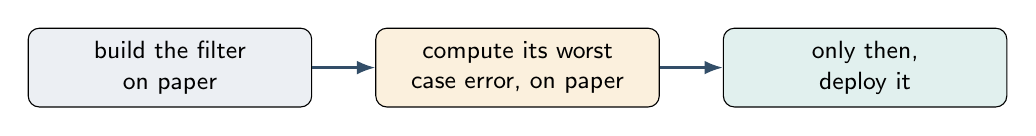
\begin{tikzpicture}[node distance=0.5cm, every node/.style={font=\small, align=center}]
    \node[draw, rounded corners, fill=cardGray, minimum width=3.6cm, minimum height=1cm] (a) {build the filter\\on paper};
    \node[draw, rounded corners, fill=cardAmber, right=0.8cm of a, minimum width=3.6cm, minimum height=1cm] (b) {compute its worst\\case error, on paper};
    \node[draw, rounded corners, fill=cardTeal, right=0.8cm of b, minimum width=3.6cm, minimum height=1cm] (c) {only then,\\deploy it};
    \draw[-{Latex}, thick, slate] (a)--(b);
    \draw[-{Latex}, thick, slate] (b)--(c);
  \end{tikzpicture}
  \end{center}
\end{frame}

% ---------------------------------------------------------------- results 1
\begin{frame}{Validation: Accuracy}
  Comparing the closed form baseline (pure math, zero data) against the calibrated version, fine tuned with a little data:

  \begin{center}
  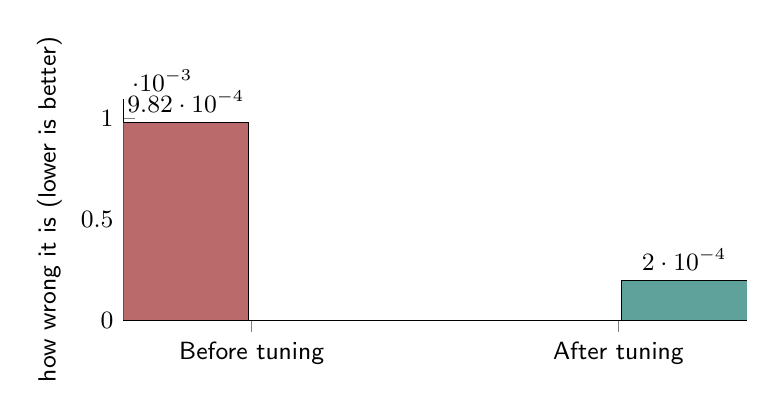
\begin{tikzpicture}
    \begin{axis}[
      width=9.5cm, height=4.4cm, ybar, bar width=1.6cm,
      symbolic x coords={Before tuning, After tuning},
      xtick={Before tuning, After tuning}, ymin=0, ymax=0.0011,
      ylabel={\small how wrong it is (lower is better)}, tick label style={font=\small},
      nodes near coords, nodes near coords style={font=\small},
      axis lines*=left, enlarge x limits=0.35
    ]
    \addplot[fill=softRed!70] coordinates {(Before tuning,9.82e-4)};
    \addplot[fill=tealAccent!70] coordinates {(After tuning,2e-4)};
    \end{axis}
  \end{tikzpicture}
  \end{center}
  \centering roughly \textbf{5 times more accurate} after the data tuning step, for no extra cost to run
\end{frame}

% ---------------------------------------------------------------- results 2
\begin{frame}{Validation: Performance}
  \begin{center}
  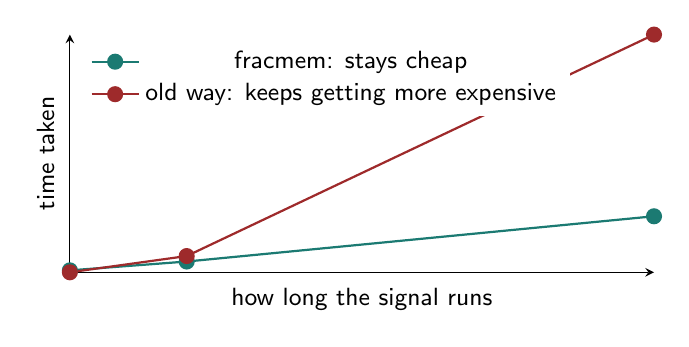
\begin{tikzpicture}
    \begin{axis}[
      width=9cm, height=4.6cm,
      xlabel={\small how long the signal runs}, ylabel={\small time taken},
      tick label style={font=\small}, label style={font=\small},
      legend style={font=\small, at={(0.02,0.98)}, anchor=north west, draw=none},
      axis lines=left, xtick=\empty, ytick=\empty
    ]
    \addplot[thick, tealAccent, mark=*, mark size=2.5pt] coordinates {(5000,8.5) (20000,34.8) (80000,169.5)};
    \addplot[thick, softRed, mark=*, mark size=2.5pt] coordinates {(5000,2.8) (20000,51.1) (80000,710.2)};
    \legend{fracmem: stays cheap, old way: keeps getting more expensive}
    \end{axis}
  \end{tikzpicture}
  \end{center}
  \centering\small\color{slate} the longer the signal runs, the bigger fracmem's advantage becomes
\end{frame}

% ---------------------------------------------------------------- hardware
\begin{frame}{Deployment Targets}
  \begin{columns}[T]
    \begin{column}{0.5\linewidth}
      \begin{center}
      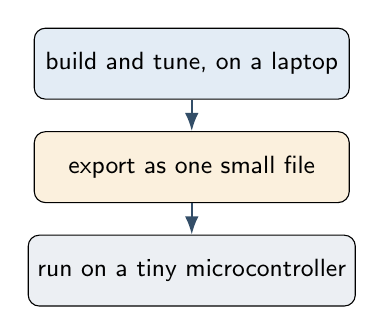
\begin{tikzpicture}[node distance=0.4cm]
        \node[draw, rounded corners, fill=cardBlue, minimum width=4cm, minimum height=0.9cm, font=\small] (fit) {build and tune, on a laptop};
        \node[draw, rounded corners, fill=cardAmber, below=of fit, minimum width=4cm, minimum height=0.9cm, font=\small] (exp) {export as one small file};
        \node[draw, rounded corners, fill=cardGray, below=of exp, minimum width=4cm, minimum height=0.9cm, font=\small] (dev) {run on a tiny microcontroller};
        \draw[-{Latex}, thick, slate] (fit)--(exp);
        \draw[-{Latex}, thick, slate] (exp)--(dev);
      \end{tikzpicture}
      \end{center}
    \end{column}
    \begin{column}{0.5\linewidth}
      \begin{itemize}
        \setlength\itemsep{0.7em}
        \item Small enough to run on a cheap microcontroller (ESP32), with no extra software installed
        \item Uses the same, tiny, fixed amount of memory whether it runs for a second or a year
        \item Useful anywhere fractional order behavior shows up: control systems, materials, batteries
      \end{itemize}
    \end{column}
  \end{columns}
\end{frame}

% ---------------------------------------------------------------- software
\begin{frame}[fragile]{Developer Interface}
  \begin{center}
  \small
  \begin{verbatim}
from fracmem import CompressedFractionalFilter

f = CompressedFractionalFilter(alpha=0.5, h=0.01, L=32, p=16)
f.fit(train_signals)          # step 3: tune with a little data
y_hat = f.predict(new_signal) # use it, on a signal of any length
  \end{verbatim}
  \end{center}
  \vspace{0.6em}
  \centering\small\color{slate} four lines: build it, tune it once, and run it
\end{frame}

% ---------------------------------------------------------------- summary
\begin{frame}{Summary}
  \begin{itemize}
    \setlength\itemsep{0.9em}
    \item Fractional order derivatives need to remember everything, forever, which naively gets more expensive the longer a system runs.
    \item fracmem remembers recent events exactly, and compresses everything older into a few fading counters, chosen by exact math.
    \item A little real data fine tunes the mix, making it about 5 times more accurate, for free.
    \item The result is provably safe to deploy, and small enough to run on a two dollar microcontroller.
  \end{itemize}
\end{frame}

% ---------------------------------------------------------------- closing / brand
{
\setbeamertemplate{footline}{}
\begin{frame}[plain]
  \vspace{1.4cm}
  \begin{center}
    {\Large\bfseries\color{inkNavy} Thank you}\\[1.4em]
    {\color{amberAccent}\rule{0.35\linewidth}{1.2pt}}\\[1.4em]
    {\huge\bfseries\color{inkNavy} adithyanlalu}\\[0.5em]
    {\small\color{slate} Adithyan Lalu \; \textbar\; Guidance, Navigation \& Control \textbar\ Autonomous Systems}\\[0.2em]
    {\small\color{slate} linkedin.com/in/adithyan-lalu}
  \end{center}
\end{frame}
}

\end{document}
